%        File: pacelc-tradeoff.tex
%     Created: July 24, 2016

\documentclass{standalone}

\usepackage{tikz}
\usepackage{tikz-qtree}
\usetikzlibrary{positioning, shapes, calc, backgrounds, fit, arrows.meta}

\renewcommand\familydefault{\sfdefault}

\begin{document}
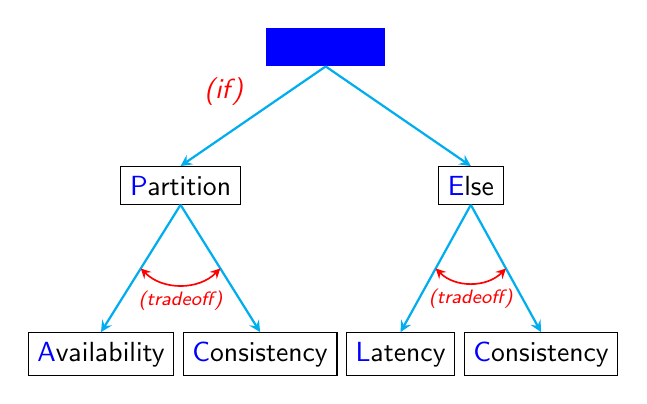
\begin{tikzpicture}[tnode/.style = {draw, rectangle},
	tedge/.style = {semithick, <->, >=stealth, red},
	tlabel/.style = {midway, yshift = -0.2cm, font = \scriptsize, red}]
  \tikzset{edge from parent/.append style = {->, >=stealth, thick, cyan}}
  \tikzset{level 1/.style={level distance = 50pt, sibling distance = 3pt}}
  \tikzset{level 2/.style={level distance = 60pt, sibling distance = 3pt}}

  \Tree 
  [.\node[draw, fill = blue!20, blue]{PACELC};
	\edge node[auto = right, red, midway] {\it (if)}; 
    [.\node[tnode]{\textcolor{blue}{P}artition}; 
	  \edge node[auto = right] (a) {};
      [.\node[tnode]{\textcolor{blue}{A}vailability};] 
	  \edge node[auto = left] (c1) {};
	  [.\node[tnode]{\textcolor{blue}{C}onsistency};] 
    ]
    [.\node[tnode]{\textcolor{blue}{E}lse}; 
	  \edge node[auto = right] (l) {};
      [.\node[tnode]{\textcolor{blue}{L}atency};] 
	  \edge node[auto = left] (c2) {};
	  [.\node[tnode]{\textcolor{blue}{C}onsistency};]
    ]
  ]

  \draw[tedge] (a) to [out = -45, in = -135] node[tlabel] {\it (tradeoff)} (c1);
  \draw[tedge] (l) to [out = -45, in = -135] node[tlabel] {\it (tradeoff)} (c2);
\end{tikzpicture}
\end{document}


